\documentclass[11pt]{book}

% Packages for Figures:
\ifx\pdftexversion\undefined
    \usepackage[dvips]{graphicx}
\else
    \usepackage[pdftex]{graphicx}
    \usepackage{epstopdf}
    \epstopdfsetup{suffix=}
\fi

% Packages for displaying code:
\usepackage{listings}
\usepackage{textcomp}
\usepackage{color}

% Color settings used in the code below:
\definecolor{dkgreen}{rgb}{0,0.6,0}
\definecolor{gray}{rgb}{0.5,0.5,0.5}
\definecolor{mauve}{rgb}{0.58,0,0.82}

% Settings for the formatting of the code on display:
\lstset{frame=tb,
  language=R,
  aboveskip=3mm,
  belowskip=3mm,
  showstringspaces=false,
  columns=flexible,
  basicstyle={\small\ttfamily},
  numbers=none,
  numberstyle=\tiny\color{gray},
  keywordstyle=\color{blue},
  commentstyle=\color{dkgreen},
  stringstyle=\color{mauve},
  breaklines=true,
  breakatwhitespace=true,
  tabsize=3
}

% Package for displaying inline verbatim commands in footnotes.
\usepackage{fancyvrb}


\begin{document}


\section*{Histogram of a Randomly Generated Variable}

We ran the following commands in R, 
displayed using the \texttt{verbatim} environment.

\begin{verbatim}
R> # Generate a random variable.
    epsilon <- rnorm(1000)

    # Plot a histogram.
    fig_ext <- 'eps'
    fig_dir <- 'Figures'
    fig_file_name <- sprintf('name_of_figure.%s', fig_ext)
    out_file_name <- sprintf('%s/%s', fig_dir, fig_file_name)

    setEPS()
    postscript(out_file_name)

    hist(epsilon, col = 'blue')

    dev.off()

\end{verbatim}

It looks boring, is not as easy to read as code in a good text editor
but it does get the message across. 


\pagebreak

Instead, we can display the code block using the 
\texttt{lstlisting} environment from the \texttt{listings} package. 

\begin{lstlisting}[language=R]
R> # Generate a random variable.
    epsilon <- rnorm(1000)

    # Plot a histogram.
    fig_ext <- 'eps'
    fig_dir <- 'Figures'
    fig_file_name <- sprintf('name_of_figure.%s', fig_ext)
    out_file_name <- sprintf('%s/%s', fig_dir, fig_file_name)

    setEPS()
    postscript(out_file_name)

    hist(epsilon, col = 'blue')

    dev.off()

\end{lstlisting}

\VerbatimFootnotes
Notice that the code above is highlighted according to the color scheme set in the \texttt{\textbackslash lstset} command in the preamble
to this document.%
\footnote{The command \texttt{\textbackslash lstset} above was displayed using the \verb|\texttt{}| command, 
with the backslash displayed using the \verb|\textbackslash| command, 
to avoid any confusion with another \LaTeX command.
In the previous sentence, 
the commands \verb|\texttt{}| and \verb|\textbackslash|
were displayed using the \verb^\verb||^
command,
which is an inline version of the \texttt{verbatim} environment.
Note that the argument of \verb+\verb||+
in the first instance of \verb^\verb||^
is enclosed in vertical bars or ``pipes'' \verb#|#
instead of braces or curly brackets \verb&{}&,
in case you want to display \LaTeX commands inline
and want to prevent any braces from interfering with
the \verb|\texttt{}| command itself.
You can also replace the pipes with many other repeated characters, 
as long as the character you choose is the first character after the \verb+\verb+ 
in the \verb+\verb{}+ command. 
%The \LaTex code for this footnote
%contains many examples of code displayed inline.
Normally, you can use the \verb+\verb+ command anywhere in 
the main text of a document;
however, the instances of \verb+\verb+ in this footnote were enabled by the 
\verb&\usepackage{fancyvrb}& package declared in the preamble
and the command \verb7\VerbatimFootnotes7
anywhere in the document before the command 
\verb!\verb! is used in a footnote. 
}



\pagebreak


\begin{figure}[h!]
\centering
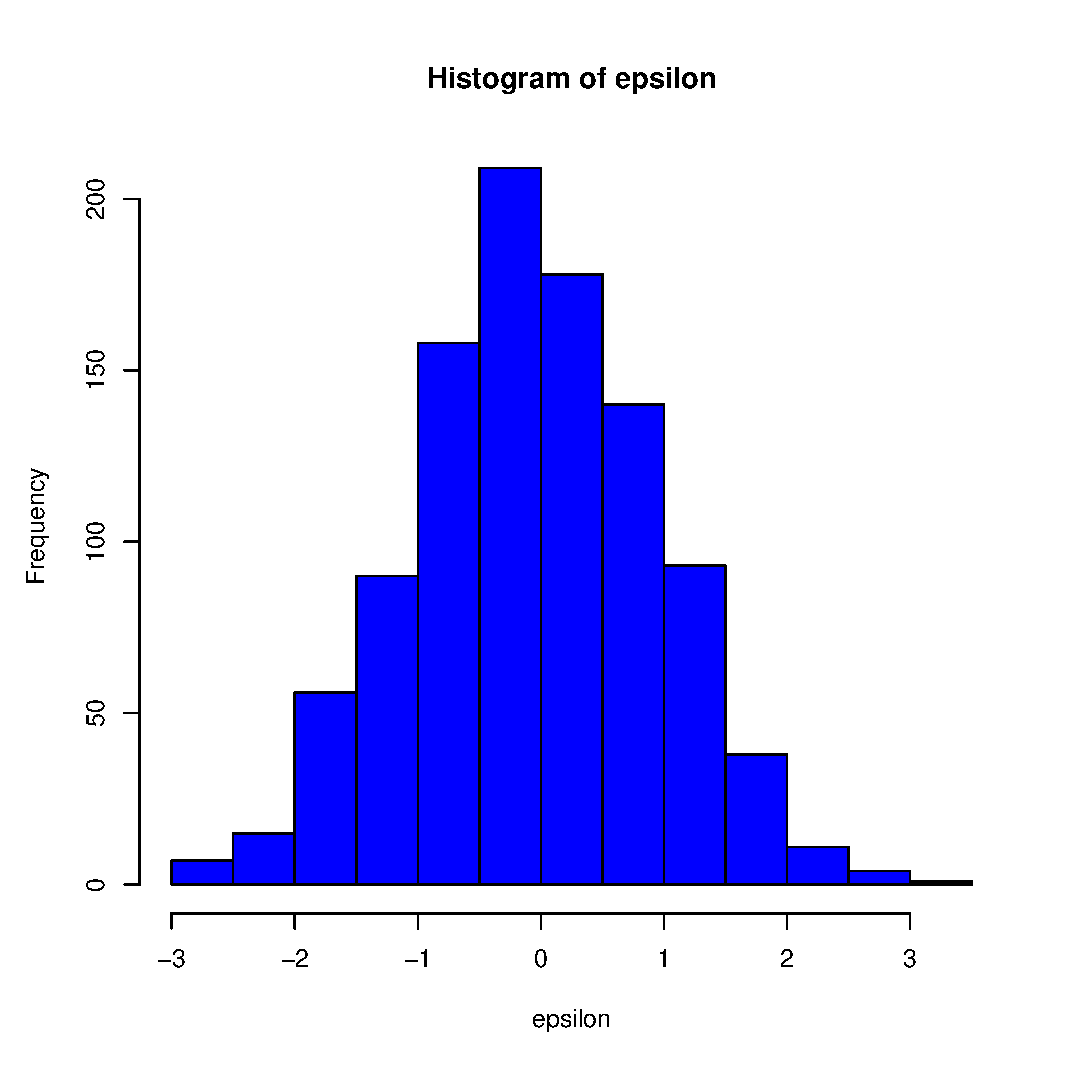
\includegraphics[width=\textwidth]{../Figures/name_of_figure.eps}
\caption{Caption Goes Here}
\label{fig:example}
\end{figure}


In any case, the histogram in Figure \ref{fig:example} shows the result of these commands.
Figures can be rendered in \LaTeX 
using the \texttt{includegraphics} command
from the \texttt{graphicx} package. 


\end{document}
